\documentclass{article}

\usepackage{graphicx}
\usepackage{amsmath}
\usepackage{fancyhdr}
\usepackage{listings}
\usepackage{xcolor}
\usepackage{textcomp}
\usepackage[sorting=none]{biblatex}
\usepackage[margin=1in]{geometry}
\usepackage[font={small,it}]{caption}
\usepackage{placeins}
\usepackage{xepersian}

%\DeclareMathOperator*{\btie}{\bowtie}
\addbibresource{bibliography.bib}
\settextfont[Scale=1.2]{B-NAZANIN.TTF}
\setlatintextfont[Scale=1]{Times New Roman}
\renewcommand{\baselinestretch}{1.5}
\pagestyle{fancy}
\fancyhf{}
\rhead{تکلیف دوم درس پایگاه داده‌ها 1}
\lhead{\thepage}
\rfoot{علیرضا ابره فروش}
\lfoot{9816603}
\renewcommand{\headrulewidth}{1pt}
\renewcommand{\footrulewidth}{1pt}
%%%%%%%%%%
\lstset
{
    language=[latex]tex,
    basicstyle=\ttfamily,
    commentstyle=\color{black},
    columns=fullflexible,
    keepspaces=true,
    upquote=true,
    showstringspaces=false,
    morestring=[s]\\\%,
    stringstyle=\color{black},
}
%%%%%%%%%%

\begin{document}
\begin{titlepage}
\begin{center}

\includegraphics[width=0.4\textwidth]{figures/IUT Logo.png}\\
        
\LARGE
\textbf{دانشگاه صنعتی اصفهان}\\
\textbf{دانشکده مهندسی برق و کامپیوتر}\\
        
\vfill
        
\huge
\textbf{عنوان: تکلیف چهارم درس ریزپردازنده}\\
        
\vfill
        
\LARGE
\textbf{نام و نام خانوادگی: علیرضا ابره فروش}\\
\textbf{شماره دانشجویی: 9816603}\\
\textbf{نیم\,سال تحصیلی: پاییز 1400}\\
\textbf{مدرّس: دکتر عارف کریمی افشار}\\
\end{center}
\end{titlepage}


%\tableofcontents
\newpage

\section{}
\begin{table}[ht]
    \centering
    \begin{tabular}{|c|c|c|}
    \hline
    \textbf{داده} & \textbf{نوع متغیر(\lr{int}، \lr{varchar}، \lr{char}، $\ldots$)}\\
    \hline
    سه حرف مخفف شده ماه‌های میلادی & \lr{char}\\
    \hline
    قیمت دلاری محصولات که همگی دو رقم اعشار دارند &\lr{numeric}\\
    \hline
    نام و نام خانوادگی کاربر & \lr{varchar}\\
    \hline
    کد ملی کاربر & \lr{char}\\
    \hline
    ذخیره قیمت لحظه‌ای ارز‌های دیجیتال دلار & \lr{numeric}\\
    \hline
    تعداد بازدید یک ویدئو & \lr{int}\\
    \hline
    \end{tabular}
    \caption{جدول شماره 1}
    \label{tab:tab1}
\end{table}


\section{}
\begin{latin}
\begin{lstlisting}
create table data
(
  month      	char(3),
  item_price    numeric(20, 2),
  name      	varchar(30) not null,
  national_id	char(10) not null,
  curr_price    numeric(20, 10),
  views_no    	int,
  primary key (national_id),
  foreign key (national_id) references users(social_number)
)
\end{lstlisting}
\end{latin}

\section{}
\subsection{}
\begin{latin}
\begin{lstlisting}
WHERE 1 <= (SELECT count(name) FROM student)
\end{lstlisting}
\end{latin}

قسمت منابع بررسی شود.

\subsection{}
\begin{latin}
\begin{lstlisting}
WHERE first_name SIMILAR TO 'me%' AND last_name SIMILAR TO '%avi'
\end{lstlisting}
\end{latin}

\subsection{}
\begin{latin}
\begin{lstlisting}
SELECT concat(first_name, last_name)
\end{lstlisting}
\end{latin}

\section{}

\subsection{}
\begin{figure}[ht]
    \centering
    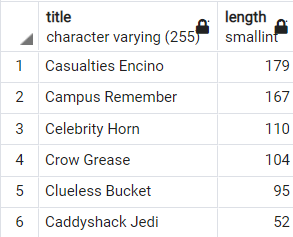
\includegraphics[width=0.3\textwidth]{figures/4-a.png}
    \caption
	{
\lr{4-a}
	}
    \label{fig:fig1}
\end{figure}

\subsection{}
\begin{figure}[ht]
    \centering
    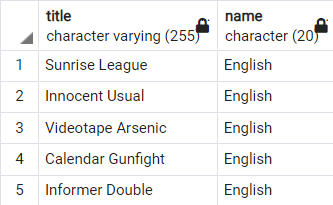
\includegraphics[width=0.3\textwidth]{figures/4-b.png}
    \caption
	{
\lr{4-b}
	}
    \label{fig:fig1}
\end{figure}

\subsection{}
\begin{figure}[ht]
    \centering
    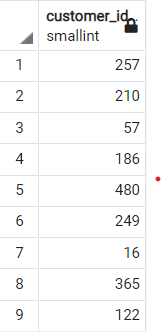
\includegraphics[width=0.3\textwidth]{figures/4-c.png}
    \caption
	{
\lr{4-c}
	}
    \label{fig:fig1}
\end{figure}

\subsection{}
\begin{figure}[ht]
    \centering
    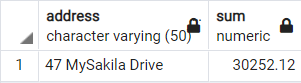
\includegraphics[width=0.3\textwidth]{figures/4-d.png}
    \caption
	{
\lr{4-d}
	}
    \label{fig:fig1}
\end{figure}

\subsection{}
\begin{figure}[ht]
    \centering
    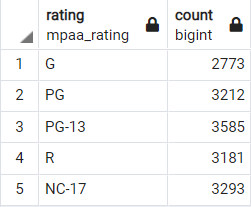
\includegraphics[width=0.3\textwidth]{figures/4-e.png}
    \caption
	{
\lr{4-e}
	}
    \label{fig:fig1}
\end{figure}

%%%%%%%%%%%%%

\section{}
\subsection{}
\begin{figure}[ht]
    \centering
    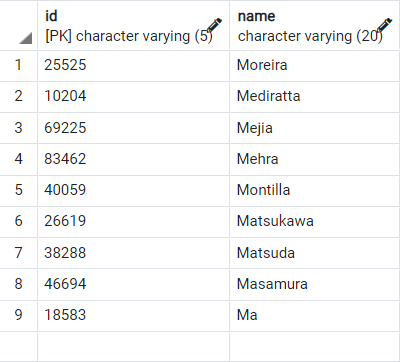
\includegraphics[width=0.3\textwidth]{figures/5-a.png}
    \caption
	{
\lr{5-a}
	}
    \label{fig:fig1}
\end{figure}

\subsection{}
\begin{figure}[ht]
    \centering
    
\includegraphics[width=0.3\textwidth]{figures/5-b.png}
    \caption
	{
\lr{5-b}
	}
    \label{fig:fig1}
\end{figure}

\subsection{}
\begin{figure}[ht]
    \centering
    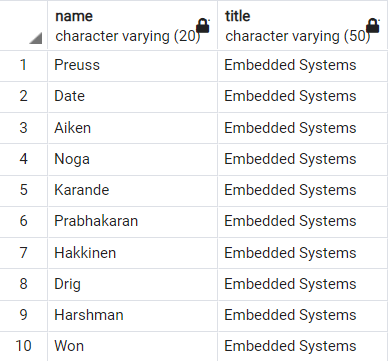
\includegraphics[width=0.3\textwidth]{figures/5-c.png}
    \caption
	{
\lr{5-c}
	}
    \label{fig:fig1}
\end{figure}

\subsection{}
\begin{figure}[ht]
    \centering
    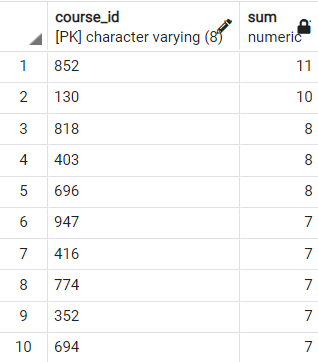
\includegraphics[width=0.3\textwidth]{figures/5-d.png}
    \caption
	{
\lr{5-d}
	}
    \label{fig:fig1}
\end{figure}

\subsection{}
\begin{figure}[ht]
    \centering
    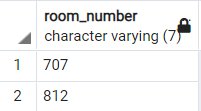
\includegraphics[width=0.3\textwidth]{figures/5-e.png}
    \caption
	{
\lr{5-e}
	}
    \label{fig:fig1}
\end{figure}

\subsection{}
\begin{figure}[ht]
    \centering
    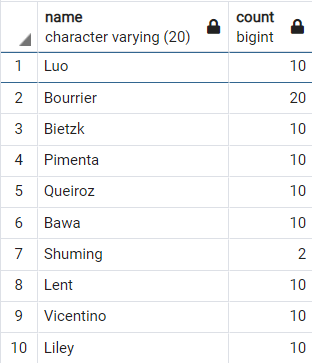
\includegraphics[width=0.3\textwidth]{figures/5-f.png}
    \caption
	{
\lr{5-f}
	}
    \label{fig:fig1}
\end{figure}

\subsection{}
\begin{figure}[ht]
    \centering
    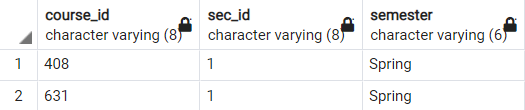
\includegraphics[width=0.3\textwidth]{figures/5-g.png}
    \caption
	{
\lr{5-g}
	}
    \label{fig:fig1}
\end{figure}

\subsection{}
\begin{figure}[ht]
    \centering
    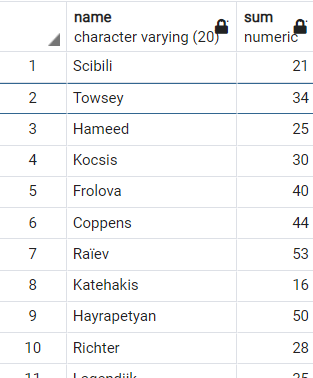
\includegraphics[width=0.3\textwidth]{figures/5-h.png}
    \caption
	{
\lr{5-h}
	}
    \label{fig:fig1}
\end{figure}


\section*{منابع}
\renewcommand{\section}[2]{}%
\begin{thebibliography}{99} % assumes less than 100 references
%چنانچه مرجع فارسی نیز داشته باشید باید دستور فوق را فعال کنید و مراجع فارسی خود را بعد از این دستور وارد کنید


\begin{LTRitems}

\resetlatinfont

\bibitem{b1} https://www.geeksforgeeks.org/sql-unique-constraint/
\end{LTRitems}

\end{thebibliography}


\end{document}
